N\documentclass{article}
\usepackage[utf8]{inputenc}
\usepackage{amstext}
\usepackage{amsmath} 
\usepackage{mathpazo}
\usepackage{textcomp}
\usepackage{graphicx} 
\usepackage{float} 
\usepackage{caption} 
\usepackage{epstopdf} 
\usepackage{hyperref}
\usepackage{varioref} 
\usepackage{fancyref}
\usepackage[section]{placeins} 
\usepackage{perpage}
\usepackage[margin=1in, paperwidth=8.5in, paperheight=11in]{geometry} 
\MakeSorted{figure} 
\usepackage{natbib}
\usepackage{graphicx}
\usepackage{xcolor}
\usepackage{listings}
\usepackage{minted}
\usepackage{subcaption}
\usepackage{eso-pic}
\usepackage{tikz}
\usepackage[american]{circuitikz}
\usepackage[font=small,labelfont=bf]{caption}

\title{ENGR2420 Lab 4: Translinear Circuits}
\author{Abigail Fry \\ Anusha Datar \\ Vienna Scheyer}
\date{March 14, 2019}

\begin{document}
\maketitle
\section{Experiment One: Bipolar Transistor Matching}
In experiment one, we measured the current-voltage characteristic of each transistor in the MAT14 quad NPN bipolar transistor array by holding the collector current at 5 Volts, sweeping the base voltage from 0.3 Volts to 0.8 Volts, and measuring both the base and emitter currents relative to ground. By measuring both the base and emitter currents and computing their difference, we could determine the change in collector current as the voltage increased.

\begin{figure}[H]   
  \centering        
  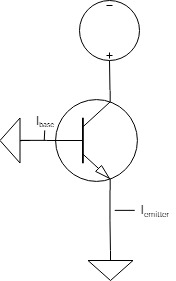
\includegraphics[scale = 0.5]{images/experiment_one_schematic.jpg}
  \caption{The schematic for the circuit used to determine the current-voltage characteristic of each transistor in the transistor array.}   
  \label{fig:exp1_sch}
\end{figure}

To track each individual transistor within the array, we labeled them Q1, Q2, Q3, and Q4 in clockwise order.

\subsection{Results}
By computing the collector current of each transistor and quantifying the relationship between the base voltage and collector current, we were able to find values for the collector saturation current, $I_s$, and the forward current gain, $\beta$ for each transistor. $\beta$ is a dimensionless ratio between currents.

\begin{table}[h]
\centering
$I_S$ and $\beta$ for MAT14 Transistors
\\
\begin{tabular}{|l|l|l|l|l|}

\hline
Transistor & $I_s$ (Amps) & $\beta_avg$    \\ \hline
Q1 & 8.39e-07&  457.69 \\ \hline
Q2 & 9.41e-07 &  428.5   \\ \hline
Q3 & 10.054e-07 &  485.10\\ \hline
Q4 & 9.53e-07 &  432.01  \\ \hline
\end{tabular}
\end{table}

We can plot the current-voltage characteristic for each of the transistors on semilogarithmic axes. Figure 2 shows a plot with all four collector currents and all four base currents as a function of the base voltage.
\begin{figure}[H]   
  \centering        
  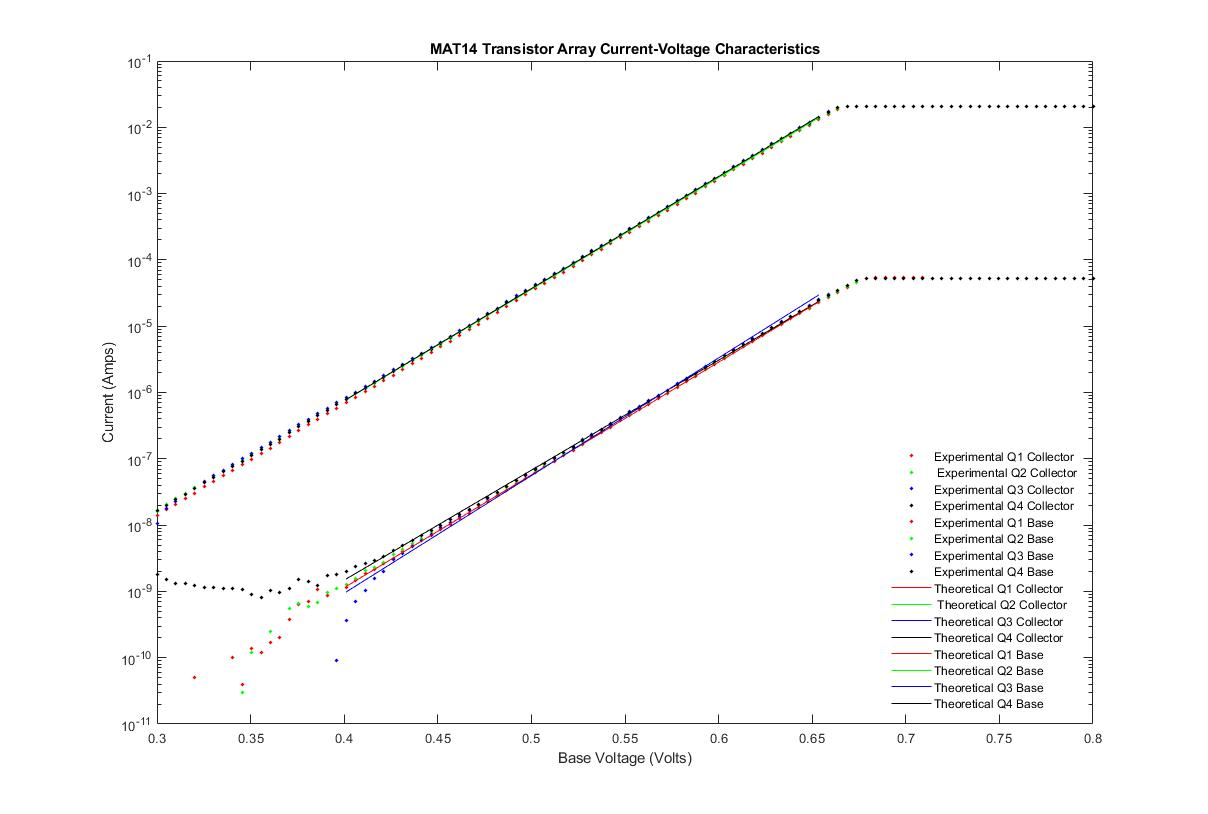
\includegraphics[scale = 0.3]{images/exp1_cv_char.jpg}
  \caption{Current-Voltage characteristic for each of the transistors in the MAT14 NPN transistor array.}   
  \label{fig:exp1_cv}
\end{figure}

To compare the four transistors in the array, we can plot the percentage difference between the collector current and the mean collector current for all of the transistors at each voltage value.
\begin{figure}[H]   
  \centering        
  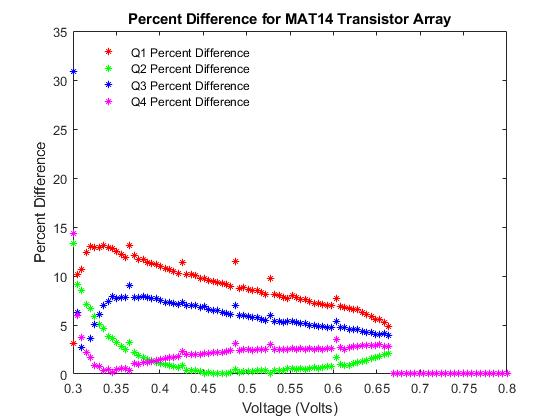
\includegraphics[scale = 0.5]{images/percent_diff.jpg}
  \caption{Percent deviation from mean collector current value for each of the transistors in the MAT14 NPN transistor array.}
  \label{fig:exp1_mean_diff}
\end{figure}

We can also examine the forward current gain, or $\beta$ value, for each of the transistors. Figure 4 shows a plot of $\beta$ as a function of base current for all four transistors.
\begin{figure}[H]   
  \centering        
  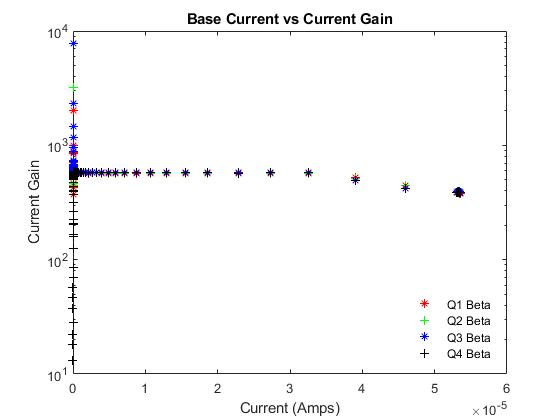
\includegraphics[scale = 0.5]{images/Beta_Exp1.jpg}
  \caption{Forward current gain, $\beta$, for each transistor as a function of the base voltage.}   
  \label{fig:exp1_beta}
\end{figure}

\subsection{Analysis}
Since instrumentation constraints prevent direct measurement of collector current, we instead measured the emitter and base currents and then calculated collector current for each of the transistors in the array.

\begin{centering}
    $$I_c = I_e - I_b$$
\end{centering}

For the theoretical current-voltage fits for the semilog and linear axes plots in Figure \ref{fig:exp1_cv}, we calculated the linear theoretical relationship of base voltage to base and emitter current using the MATLAB $polyfit$ function. 
From this fit, we extracted the saturation current, $I_s$, by calculating the exponential of the intercept of a $polyfit$ to the linear part of the semilog plotted current-voltage characteristic. For the average $\beta$ value of each transistor, we calculate $\beta$ at each set of sampled current values and then calculate the average of those $\beta$ values by dividing the sum of all of the $\beta$ values by $i$, the number of $I_c$ values sampled. To calculate $\beta$ for the current vs. $\beta$ plot in Figure \ref{fig:exp1_beta}, we plotted the base current (in Amps) on the x axis and the $\beta$ values for each transistor at each base current on the y axis.

\begin{centering}
    $$\beta = \frac{I_{c}}{I_{b}}$$
    \newline
    $$\beta_{avg} = \frac{\Sigma\beta_{i}}{i}$$
\end{centering}


To calculate the percent difference for between individual collector currents and the mean collector current for the transistor array, we first found the mean collector current.

\begin{centering}
    $$I_{c_{avg}}= \frac{I_{c_{Q1}} + I_{c_{Q2}} + I_{c_{Q3}} + I_{c_{Q4}}}{4} $$
\end{centering}

Then, we found the percent difference for each of the four transistors in the array where $n$ is the transistor number.

\begin{centering}
    $$  I_{cn{_{diff}}} = \frac{|I_{c_n} - I_{c_{avg}}|} {{\frac{I_{c_n} + I_{c_{avg}}}{2}}}$$
\end{centering}

\subsection{Discussion}
The transistors in the MAT14 array match one another very well - this  makes sense because the 4 transistors are in an integrated chip and are supposed to have identical behaviors.  The current-voltage characteristics in Figure \ref{fig:exp1_cv} shows that all four transistors follow a very similar trend at both the base current and collector current. The extracted $I_{s}$ values have a variation of \textpm  $2 $x$ 10^{-7}$, which is trivial considering the order of magnitude.  The base current vs $\beta$ plot in Figure \ref{fig:exp1_beta} shows that all four transistors show the same change in current gain values as a function of base voltage.  The average value of $\beta_{avg}$ is 450.83 - all of the extracted values of $\beta_{avg}$ are within 7.6\% of this average. While all of the transistors behave consistently, we can examine systematic trends in the differences between them with the percent difference plot in Figure \ref{fig:exp1_mean_diff}- each of the transistors has its own consistently different percent deviation from the average between 0.3 and 0.65 Volts, and then all of the transistors have very little change from the average at voltages greater than 0.65.  
\newline
\newline
\section{Experiment Two: Translinear Circuit One}
In experiment two, we measured the output current, $I_z$, as a function of both the source current, $I_x$, and the sink current, $I_y$. Because we only have two channels on our SMU, we could not directly control both the source and sink currents and also measure the output current, $I_z$, so we constructed fixed current source and fixed current sink circuits. Then, we could sweep $I_x$, hold $I_y$ constant, and measure $I_z$. By varying a resistor value in the sink circuit, we can change the value of $I_y$ and study how that impacts $I_z$. After that, we could sweep $I_y$, hold $I_x$ constant, and measure $I_z$. As before, we can vary a resistor value in the source circuit to study how that impacts $I_z$.

\begin{figure}[H]   
  \centering
  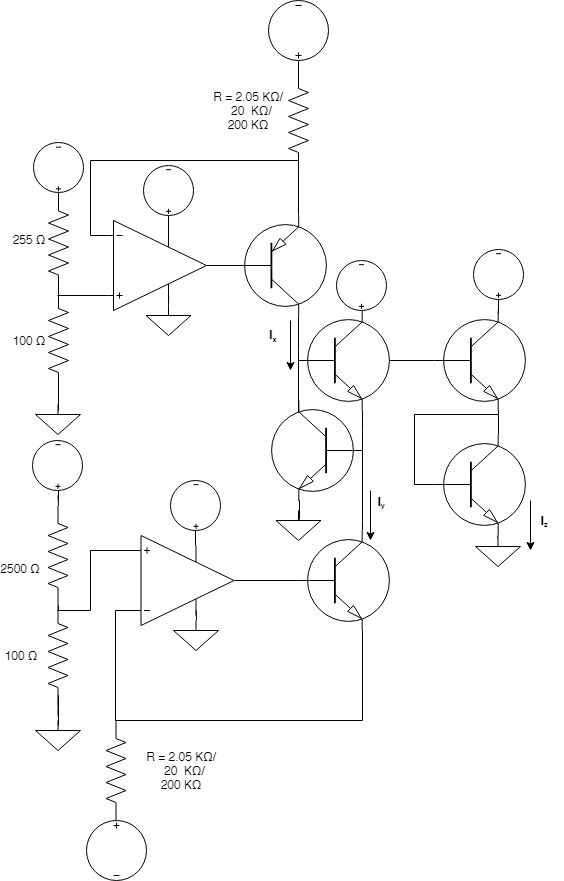
\includegraphics[scale = 0.5]{images/experiment_two_schematic.jpg}
  \caption{Translinear Circuit One. Only either the source OR the sink circuit is connected to the npn transistor loop circuit at any given time.}  
  \label{fig:exp2_sch}
\end{figure}

\subsection{Results}
We first examined the relationship between $I_x$ and $I_z$ by holding the sink current constant at .00002 Amps, .000002 Amps, and .0000002 Amps by using 10K$\Omega$, 100K$\Omega$, and 1M$\Omega$ resistors in our sink circuit. 
\begin{figure}[H]
  \centering        
  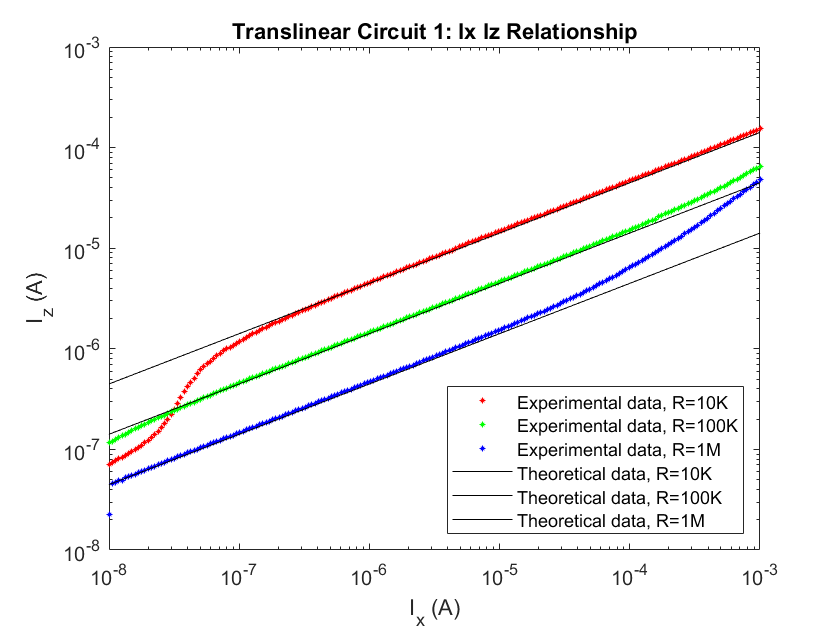
\includegraphics[scale = 0.5]{images/Exp3_Ix_plot.png}
  \caption{Translinear Circuit Two $I_x$/$I_z$ relationship.} 
  \label{fig:exp2_ixiz}
\end{figure}

We then studied the relationship between $I_y$ and $I_z$ by holding the source current constant at .00025 Amps, .000025 Amps, and .0000025 Amps by using 10K$\Omega$, 100K$\Omega$, and 1M$\Omega$ resistors in our source  circuit. 
\begin{figure}[H]   
  \centering        
  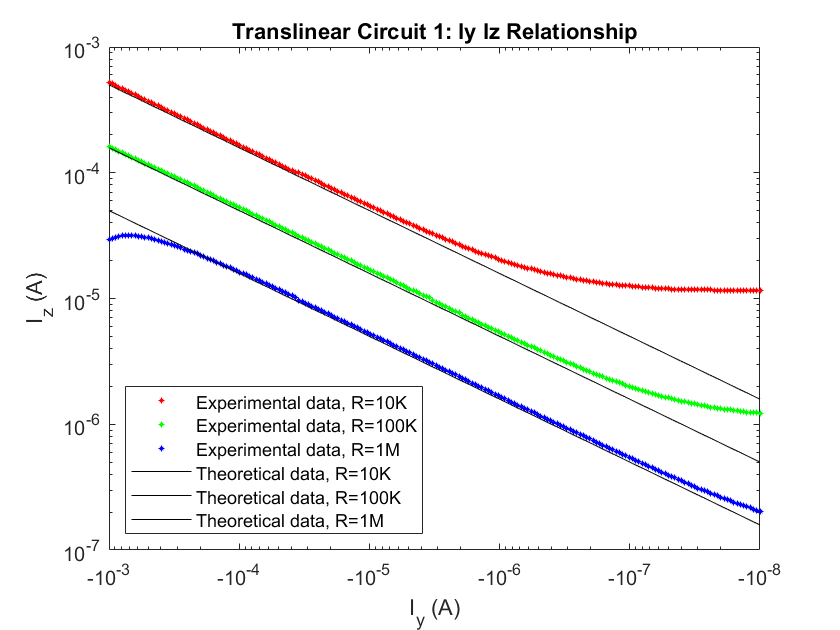
\includegraphics[scale = 0.5]{images/Exp2_Iy_plot.png}
  \caption{Translinear Circuit Two $I_y$/$I_z$ relationship.} 
  \label{fig:exp1_ixiz}
\end{figure}

\subsection{Analysis}
For the theoretical fits, we used the translinear principle from the prelab

\begin{centering}
$$I_1 I_2 = I_3 I_4$$
\end{centering}

When we apply this principle to the circuit in Figure 5, we get the following equation

\begin{centering}
$$I_x I_y = I_x ^2$$
\end{centering}

Solving for $I_z$, we get

\begin{centering}
$$I_z = \sqrt{I_x I_y}$$
\end{centering}

To get the $I_x$ $I_z$ relationship, we swept $I_y$ from 10nA to 10mA. We repeated this $I_y$ sweep for 3 different values of $I_x$ that we calculated using Ohm's law, 0.00002A, and 0.000002A, 0.000002A.

Since we are plotting the experimental data on loglog axes, we manipulate the equation into the following logarithmic slope-intercept form

\begin{centering}
$$log(I_z) = \frac{1}{2} log(I_x) + \frac{1}{2} log(I_y)$$
\end{centering}

When we are sweeping values for $I_x$ and holding $I_y$ constant at 3 different values, as shown in Figure 6, the $I_x$ term coefficient in the above equation tells us the slope, which is $\frac{1}{2}$, and the $log(I_y)$ term tells us the y-intercept in Amps. Table 1 shows the expected and actual slopes for the $I_x$ $I_z$ relationship with percent errors.
Table 2 shows the expected and actual y-intercepts for the $I_x$ $I_z$ relationship with percent errors.

When we sweep values for $I_y$ and hold $I_x$ constant at 3 different values, the roles of these terms switch. The slopes should also be $\frac{1}{2}$, and the y-intercepts are determined by the $I_x$ term (in Amps).
Table 3 shows the expected and actual slopes for the $I_y$ $I_z$ relationship with percent errors.
Table 4 shows the expected and actual y-intercepts for the $I_y$ $I_z$ relationship with percent errors.
We used the $polyfit$ function in MATLAB to find the slope of the linear portions of our data. 

\begin{table}[h]
    \centering
    \begin{tabular}{|c|c|c|c|}
        \hline
        Current (Amps) & Expected Slope & Actual Slope & Slope Percent Error \\
        
         0.00002 & 0.5 & 0.5050 & 0.5\% \\ \hline
         0.000002 & 0.5 & 0.5040 & 0.4\% \\ \hline 
         0.0000002 & 0.5 & 0.5066 & 0.66\% \\ \hline 
    \end{tabular}
    \caption{Expected and Actual slopes with percent error for Translinear Circuit 1 $I_x$ $I_z$ relationship}
    \label{tab:my_label}
\end{table}

\begin{table}[h]
    \centering
    \begin{tabular}{|c|c|c|c|}
        \hline
        Current (Amps) & Expected y-intercept & Actual y-intercept & y-intercept Percent Error \\
        
         0.00002 & -5.410A & -5.311A & 9.9\% \\ \hline
         0.000002 & -6.561A & -6.477A & 8.4\% \\ \hline 
         0.0000002 & -7.713A & -7.577A & 13.6\% \\ \hline 
    \end{tabular}
    \caption{Expected and Actual slopes with percent error for Translinear Circuit 1 $I_x$ $I_z$ relationship}
    \label{tab:my_label}
\end{table}

\begin{table}[h]
    \centering
    \begin{tabular}{|c|c|c|c|}
        \hline
        Current (Amps) & Expected Slope & Actual Slope & Slope Percent Error \\
        
         0.00025 & 0.5 & 0.4996 & 0.04\% \\ \hline
         0.000025 & 0.5 & 0.4909 & 0.91\% \\ \hline 
         0.0000025 & 0.5 & 0.4972 & 0.28\% \\ \hline 
    \end{tabular}
    \caption{Expected and Actual slopes with percent error for Translinear Circuit 1 $I_y$ $I_z$ relationship}
    \label{tab:my_label}
\end{table}

\begin{table}[h]
    \centering
    \begin{tabular}{|c|c|c|c|}
        \hline
        Current (Amps) & Expected y-intercept & Actual y-intercept & y-intercept Percent Error \\
        
         0.00025 & -4.147A & -4.102A & 4.5\% \\ \hline
         0.000025 & -5.238A & -5.332A & 9.4\% \\ \hline 
         0.0000025 & -6.451A & -6.431A & 2\% \\ \hline 
    \end{tabular}
    \caption{Expected and Actual slopes with percent error for Translinear Circuit 1 $I_y$ $I_z$ relationship}
    \label{tab:my_label}
\end{table}
\newpage
\subsection{Discussion}
The behavior of the circuit reflects the equation from the prelab analysis in the section where it shows linear behavior - as predicted, lines fit to the linear section of the $I_x$ $I_z$ graph approximately have a slope of $\frac{1}{2}$ and a y-intercept of $\frac{1}{2}log(I_y)$ Amps, and lines fit to the linear section of the $I_y$ $I_z$ graph approximately have a slope of $\frac{1}{2}$ and a y-intercept of $\frac{1}{2}$ Amps with minimal percent error.

The more interesting deviation involves the sections of the graph where the current ratio does not display linear behavior - namely at the bounds of the current ranges. This nonlinear behavior is likely due to fluctuating base currents not accounted for in the equation that can become exaggerated at dramatic current ratios. After all, even though theoretical calculations assume there is no base current and that $\beta$ is infinite, our plots from Experiment One prove that this is not the case. Because of this effect, the error becomes more apparent for $I_y$ when $I_x$ is higher, and it becomes more visible for $I_x$ when $I_y$ is lower.  

\section{Experiment Three: Translinear Circuit Two}
In experiment three, we measured the output current, $I_z$, as a function of both the source current, $I_x$, and the sink current, $I_y$. Because we only have two channels on our SMU, we could not directly control both the source and sink currents and also measure the output current, $I_z$, so we constructed fixed current source and current sink circuits. Then, we could sweep $I_x$, hold $I_y$ constant, and measure $I_z$ - by varying a resistor value within the sink circuit, we can change the value of $I_y$ and study how that impacts $I_z$. After that, we could sweep $I_y$, hold $I_x$ constant, and measure $I_z$ - similarly, we can vary a resistor value in the source circuit to study how changes in $I_x$ impact $I_z$.

\begin{figure}[H]   
  \centering        
  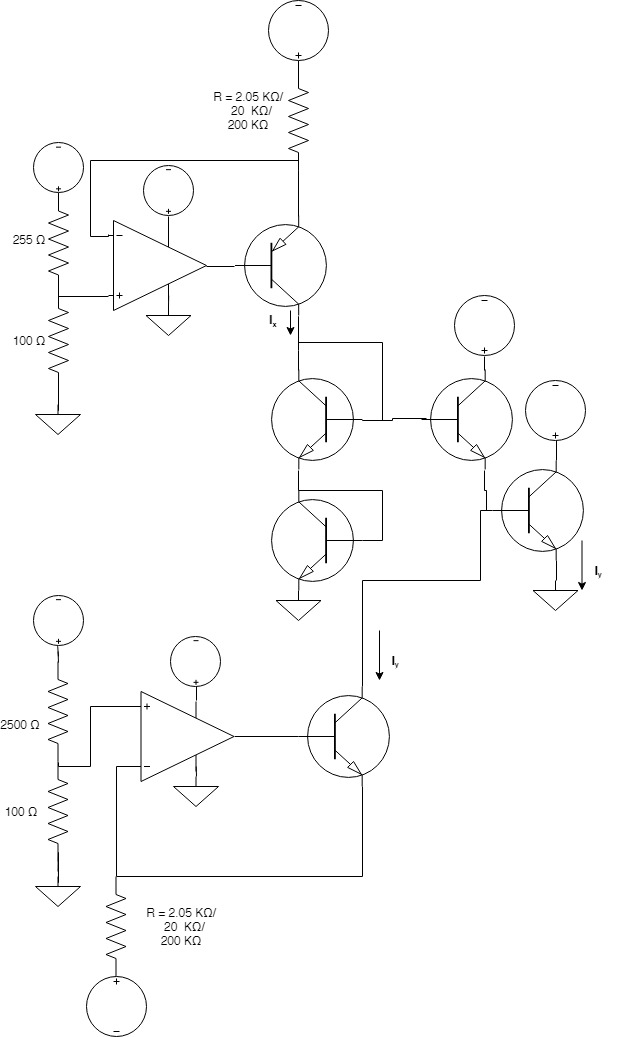
\includegraphics[scale = 0.5]{images/experiment_three_schematic.jpg}
  \caption{Translinear Circuit 2. Only either the source OR the sink circuit is connected to the npn transistor loop circuit at any given time.} 
  \label{fig:exp1_sch}
\end{figure}

\subsection{Results}
We first examined the relationship between $I_x$ and $I_z$ by holding the sink current constant at .00002 Amps, .000002 Amps, and .0000002 Amps by using 10K, 100K, and 1M$\Omega$ resistors in our sink circuit. 
\begin{figure}[H]   
  \centering        
  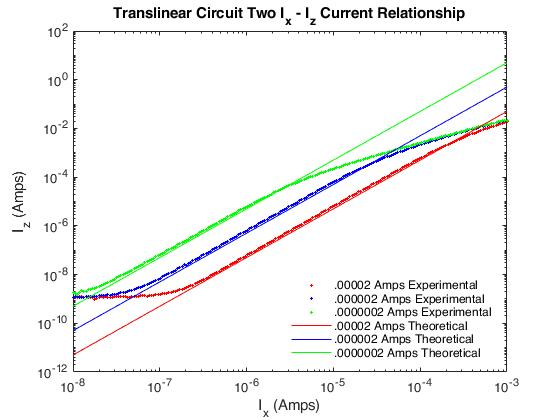
\includegraphics[scale = 0.5]{images/exp3_plot1.jpg}
  \caption{Translinear Circuit Two $I_x$ $I_z$ relationship.} 
  \label{fig:exp1_ixiz}
\end{figure}

We then studied the relationship between $I_y$ and $I_z$ by holding the source current constant at .00025 Amps, .000025 Amps, and .0000025 Amps by using 10K, 100K, and 1M$\Omega$ resistors in our source circuit. 
\begin{figure}[H]   
  \centering        
  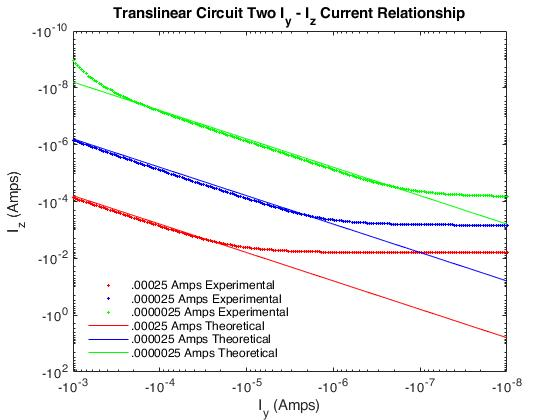
\includegraphics[scale = 0.5]{images/exp3_plot2.jpg}
  \caption{Translinear Circuit Two $I_y$ $I_z$ relationship.} 
  \label{fig:exp1_ixiz}
\end{figure}

\subsection{Analysis}
In this circuit, all four of the transistors are generally operating in the forward active mode, and the circuit forms a second-order translinear loop. This implies that the product of the currents on the right side of the loop will be equal to the product of the currents on the left side of the loop. So, nominally, 
\begin{center}
    $I_xI_x = I_yI_z$
\end{center}
\\
Therefore, we can model the relationship between $I_z$ and $I_x$ and $I_y$ as 
\begin{center}
    $I_z = \frac{(I_x)^2}{I_y}$
\end{center}
\\
So, on a log scale:
\begin{center}
    log($I_z) = 2log(I_x) - log({I_y})$
\end{center}
\\
This model implies that each of the lines in the $I_x$-$I_z$ plot should have a slope of 2 and a y-intercept of $log(I_y)$ Amps. By plotting the relationship between $I_x$ and $I_z$ for each value of $I_y$ and using MATLAB's $polyfit$ function, we can determine the slope and intercepts of the linear portion of each graph. After determining these values, we can calculate the percent error by computing the quotient of the difference between the experimental and theoretical value and the theoretical value. Note that the slope is a dimensionless quantity because it is the ratio of two current values.
\\
\newline
\begin{table}[h]
    \centering
    \begin{tabular}{|c|c|c|c|}
        \hline
        Current (Amps) & Expected Slope & Actual Slope & Slope Percent Error \\ \hline
        0.00002 & 2 & 1.97 & 1.5\%  \\ \hline
        0.000002 & 2 & 1.98 & 1\% \\  \hline 
        0.0000002 & 2 & 1.97 & 1.5\% \\ \hline
    \end{tabular}
    \caption{The slope of the $I_x$  $I_z$ plot for experiment three.}
    \label{tab:my_label}
\end{table}

\begin{table}[h]
    \centering
    \begin{tabular}{|c|c|c|c|}
        \hline
        Current (Amps) & Expected Y-Intercept (Amps) & Actual Y-Intercept (Amps) & Y-Intercept Percent Error \\ \hline
        0.00002 & 10.82 & 10.70 & 1.1\%  \\ \hline
        0.000002 & 13.12 & 13.04 & 0.1\% \\  \hline 
        0.0000002 & 15.42 & 15.22 & 1.2\% \\ \hline
    \end{tabular}    
    \caption{The y-intercepts data of the $I_x$ $I_z$ plot for experiment three.}
    \label{tab:my_label}
\end{table}

Furthermore, we also know that each of the lines in the $I_y$-$I_z$ plot should have a slope of -1 and a y-intercept of $2log(I_y)$ Amps. By plotting the relationship between $I_x$ and $I_z$ for each value of $I_y$ and using MATLAB's $polyfit$ function, we can determine the slope and intercepts of the linear portion of each graph. After determining these values, we can calculate the percent error by computing the quotient of the difference between the experimental and theoretical value and the theoretical value.

\\
\begin{table}[h]
    \centering
    \begin{tabular}{|c|c|c|c|}
        \hline
        Current (Amps) & Expected Slope & Actual Slope & Slope Percent Error \\ \hline
        0.00025 & -1 & -0.98 & 2\%  \\ \hline
        0.000025 & -1 & -0.95 & 5\% \\  \hline 
        0.0000025 & -1 & -1.05 & 5\% \\ \hline
    \end{tabular}
    \caption{The slope of the $I_y$ $I_z$ plot for experiment three.}
    \label{tab:my_label}
\end{table}
\\
\begin{table}[h]
    \centering
    \begin{tabular}{|c|c|c|c|}
        \hline
        Current (Amps) & Expected Y-Intercept (Amps) & Actual Y-Intercept (Amps) & Y-Intercept Percent Error \\ \hline
        0.00025 & -16.59 & -16.32 & 1.6\%  \\ \hline
        0.000025 & -21.19 & -20.95 & 1.1\% \\  \hline 
        0.0000025 & -25.80 & -26.22 & 1.6\% \\ \hline
    \end{tabular}    
    \caption{The y-intercept data of the $I_y$ $I_z$ plot for experiment three.}
    \label{tab:my_label}
\end{table}

\subsection{Discussion}
The behavior of the circuit reflects the equation from the prelab analysis in the section where it shows linear behavior. As predicted, lines fit to the linear section of the $I_x$ $I_z$ graph approximately have a slope of 2 and a y-intercept of $log(I_y)$ Amps, and lines fit to the linear section of the $I_y$ $I_z$ graph approximately have a slope of -1 and a y-intercept of $2log(I_x)$ Amps with minimal percent error.

The more interesting deviation involves the sections of the graph where the current ratio does not display linear errors - namely at the bounds of the current ranges. This nonlinear behavior is likely due to fluctuating base currents not accounted for in the equation that can become exaggerated at dramatic current ratios. After all, even though theoretical calculations assume there is no base current and that $\beta$ is infinite, our plots from Experiment One prove there is a small amount. Because of this effect, the error becomes more apparent for $I_y$ when $I_x$ is higher, and it becomes more visible for $I_x$ when $I_y$ is lower.  
\end{document}
